
	\documentclass{article}
	\usepackage{amsmath,amssymb}
	\usepackage[inline]{enumitem}
	\usepackage{blindtext}
	\usepackage{booktabs}
	\usepackage{graphicx}
	\usepackage{xcolor}
	\usepackage[vmargin = 1.5in, top = 1in, bottom = 1.2in, letterpaper]{geometry}
	\usepackage{listings}
	\usepackage{courier}
	\usepackage{multicol}
	\usepackage{multirow}
	\usepackage{bm}
	\usepackage{algorithm}
	\usepackage{algpseudocode}
	\usepackage{subfigure}
	\usepackage{appendix}
	\lstset{
	basicstyle = \small\tt,
	keywordstyle = \ttfamily\bfseries\color{blue},
	commentstyle = \it\color[cmyk]{1,0,1,0},
	stringstyle = \tt\color[RGB]{128,0,0},
	%frame = single,
	backgroundcolor = \color[RGB]{245,245,244},
	breaklines,
	extendedchars = false,
	xleftmargin = 2em,
	xrightmargin = 2em,
	aboveskip = 1em,
	tabsize = 4,
	showspaces = false
	showstringspaces = false
	}

	\setlength{\parindent}{0em}
	\setlength{\parskip}{1em}
	\begin{document}
	
	% \newfontfamily\courier{Courier New}

	
	\title{\bf STAT 580 Final Report}
	\author{Yifan Zhu, Gang Han, Lijin Zhang, Lingnan Yuan\\ \  \\ \textit{Department of Statistics, Iowa State University}}
	\date{}
	\maketitle
	
	\section{Summary of Soft-Impute}
First we want to fit a matrix $\widehat{\mathbf{Z}}$ that approximates $\mathbf{Z}$ in a suitable sense. By doing this, we can find an approximation that has simple structure or fill in any missing entries in $\mathbf{Z}$ which is our purpose.\cite{hastie2015statistical}

Our general approach is to consider estimators based on optimization problem of the form:
\begin{equation}\label{original}
\widehat{\mathbf{Z}}= \arg \min_{\mathbf{M}\in \mathbb{R}^{m\times n}} \| \mathbf{Z} - \mathbf{M} \|^2_F \qquad \textrm{subject to} \qquad\Phi(\mathbf{M})\le c,
\end{equation}
$\Phi(\cdot)$ is a constraint function that encourages $\hat{\mathbf{Z}}$ to be sparse in some general sense. There are some kinds of constraint methods, one is the singular value decomposition that we'll discuss later.

The SVD provides a solution to the rank-q matrix matrix approximation problem. Then our optimization problem (\ref{original}) has the form:
\begin{equation}
\arg\min_{rank(\mathbf{M}) = r} \| \mathbf{Z} - \mathbf{M} \|_F.
\end{equation}

It has a closed form solution $\widehat{\mathbf{Z}}_r = UD_rV^T$. It's sparse in the sense that all but r singular values are 0 and it provides an effective method for matrix completion.

Suppose our observed entries of the matrix $\mathbf{Z}$ indexed by the subset $\Omega \subset \{1,\cdots,m\}\times \{1,\cdots,n\}$. A natural approach is to seek the lowest rank approximating matrix $\widehat{\mathbf{Z}}$.
But forcing the estimate $\mathbf{M}$ to interpolate each of the observed entries $z_{ij}$ will be too harsh and can lead to overfitting. So it would be better to allow some errors. Consider the optimization problem:

\begin{equation}\label{errorversion}
\arg \min_{\mathrm{rank}(\mathbf{M})\le r} \sum_{(i,j) \in \Omega}(z_{ij} - m_{ij})^2.
\end{equation}

However, the optimization problem (\ref{errorversion}) is nonconvex, the exact solutions are in general not available. The nuclear norm is a convex relaxation of the rank of a matrix, so we can give a convex relaxation with noise:

\begin{equation}
\arg \min_{\mathbf{M}} \left\{ \frac{1}{2}\sum_{(ij) \in \Omega}(z_{ij}-m_{ij})^2 + \lambda \| \mathbf{M} \|_{\ast}  \right\}.
\end{equation}

Then we can use Soft-Impute Algorithm to solve this problem.

	\begin{algorithm}
		\caption{SOFT-IMPUTE FOR MATRIX COMPLETION\cite{mazumder2010spectral}}
		\begin{algorithmic}[1]
			\State Initialize $Z^{\mathrm{old}} = 0$ and create a decreasing grid $\lambda_1>\cdots > \lambda_n$
			\For {each $k=1,\cdots , K,$ set $\lambda = \lambda_k$ and iterate until convergence:}
			\State {Compute $\widehat{\mathbf{Z}}_{\lambda}\leftarrow S_{\lambda}(P_{\Omega}(\mathbf{Z} )+ P_{\Omega}^{\perp}(Z^{\mathrm{old}}))$.}
            \State {Update $Z^{\mathrm{old}} \leftarrow \widehat{\mathbf{Z}}_{\lambda}$}
			\EndFor
            \State {Output the sequence of solutions $\widehat{\mathbf{Z}}_{\lambda_1},\cdots,\widehat{\mathbf{Z}}_{\lambda_K}$.}
		\end{algorithmic}
	\end{algorithm}

Define the projection operator $P_{\Omega}:\mathbb{R}^{m\times n} \mapsto \mathbb{R}^{m\times n}$ as follows:
\begin{equation}
[P_{\Omega}(\mathbf{Z})]_{ij} = \begin{cases}
z_{ij}  \qquad & \mathrm{if} \quad (i,j)\in\Omega\\
0 \qquad & \mathrm{if} \quad (i,j) \notin \Omega
\end{cases}
\end{equation}

Define the soft-thresholded version of SVD as:
\begin{equation}
S_{\lambda}(\mathbf{W}) \equiv \mathbf{UD_{\lambda}V^T} \quad \mathrm{where} \quad \mathbf{D_{\lambda}} = \mathrm{diag}[(d_1 - \lambda)_{+},\cdots,(d_r - \lambda)_{+}].
\end{equation}

	\section{Comparison of SVD implementations}
We've got different functions of doing soft-impute implementations using 4 svd methods. Now we want to compare which of these methods is the fastest and which of these methods is the most accurate.

First of all, we simulated several matrices using the underlying model:

$$
\mathbf{Z}_{m\times n} = \mathbf{U_{m\times  r}V^{T}_{r\times n} + \epsilon}
$$

Where $\mathbf{U}$ and $\mathbf{V}$ are random matrices with standard normal Gaussian entries, and $\epsilon $ is i.i.d. Guassian. $\Omega$ is uniformly random over the indices of the matrix with p $\%$ of missing entries.
Define the SNR, test error and training error as:
$$
\textrm{SNR} = \sqrt{\frac{\mathrm{var}(UV^T)}{\mathrm{var}(\epsilon)}}
$$
$$
\textrm{Test error} = \frac{\| P^{\perp}_{\Omega}(UV^T - \widehat{Z}) \|^2_F}{\| P^{\perp}_{\Omega}(UV^T) \|^2_F}
$$
$$
\textrm{Training error} = \frac{\| P_{\Omega}(Z - \widehat{Z}) \|^2_F}{\| P_{\Omega}(Z) \|^2_F}
$$

In the following figures, we show the training and test error for the 4 methods as a function of rank.

\begin{figure}[!htb]
  \centering
  \subfigure[Test error]{
    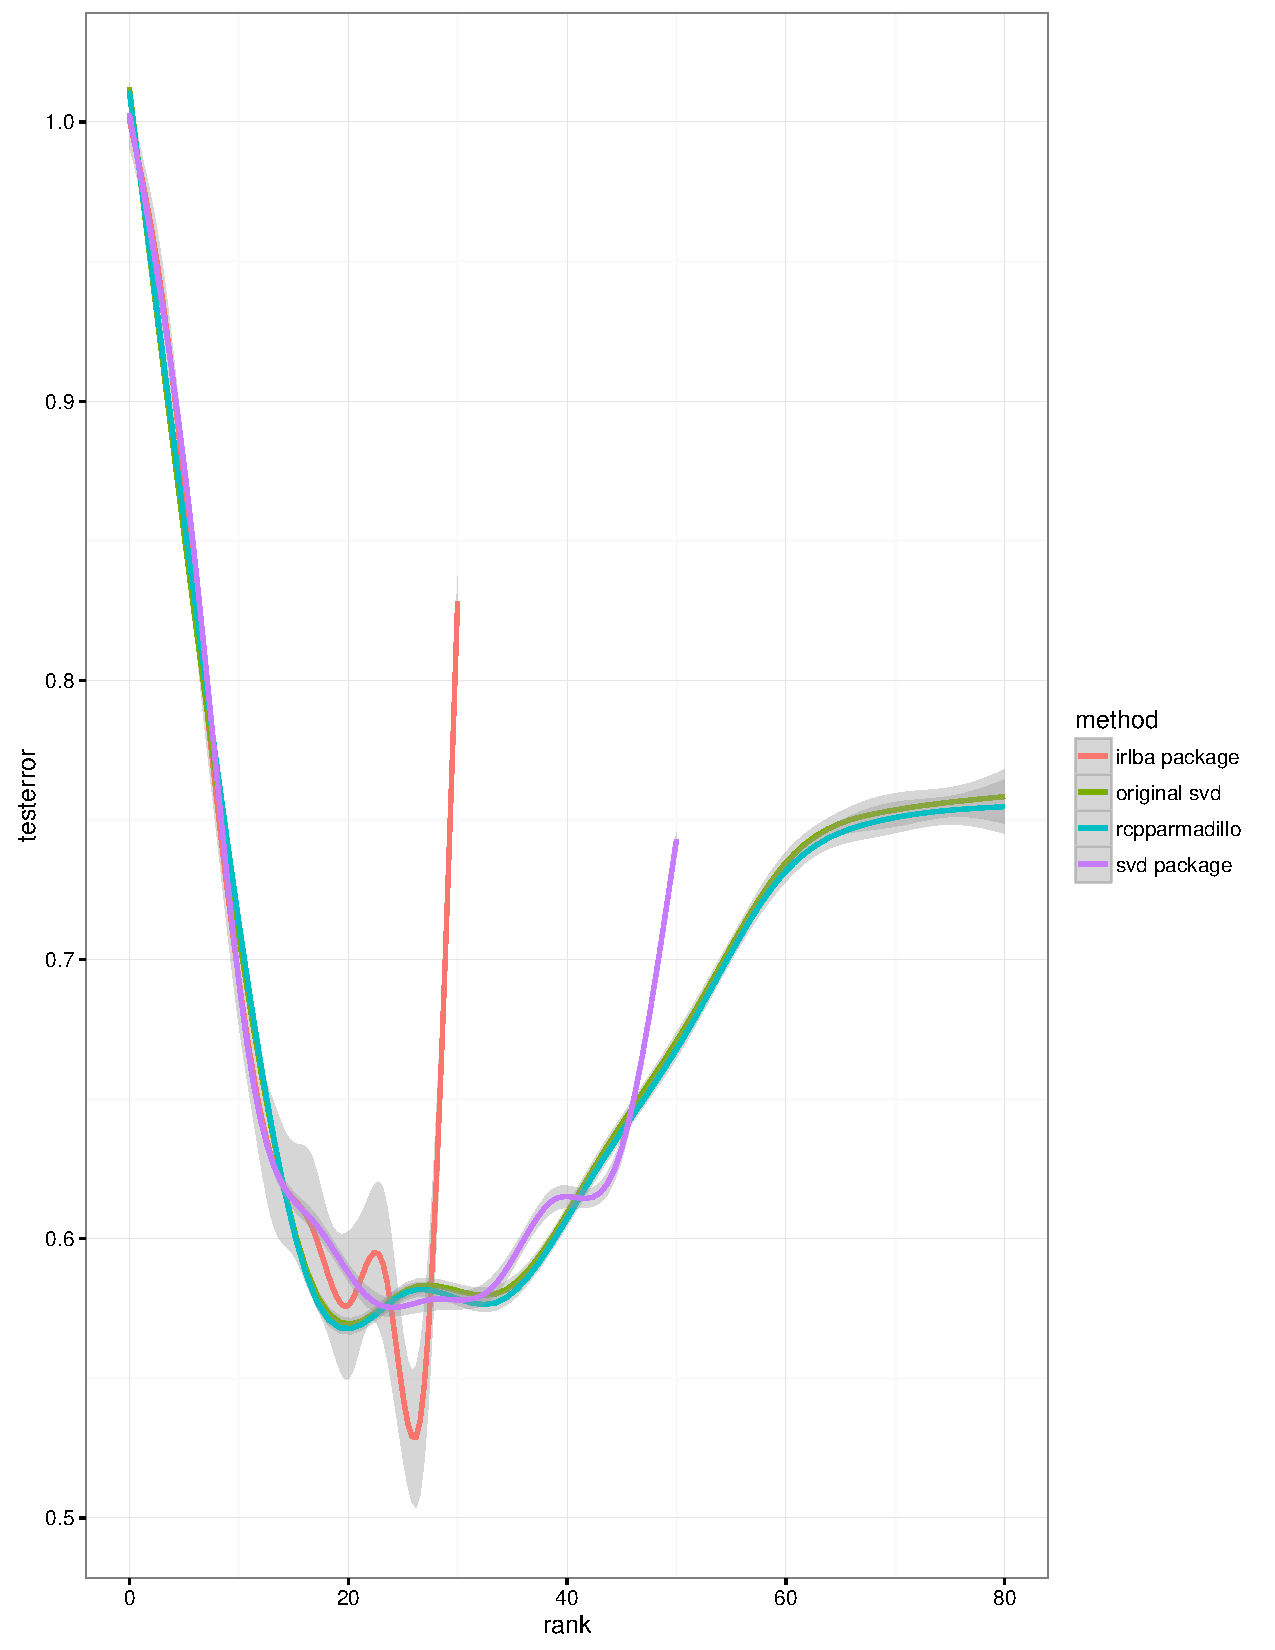
\includegraphics[width=0.45\textwidth]{testerror.pdf}}
~
  \subfigure[Training error]{
    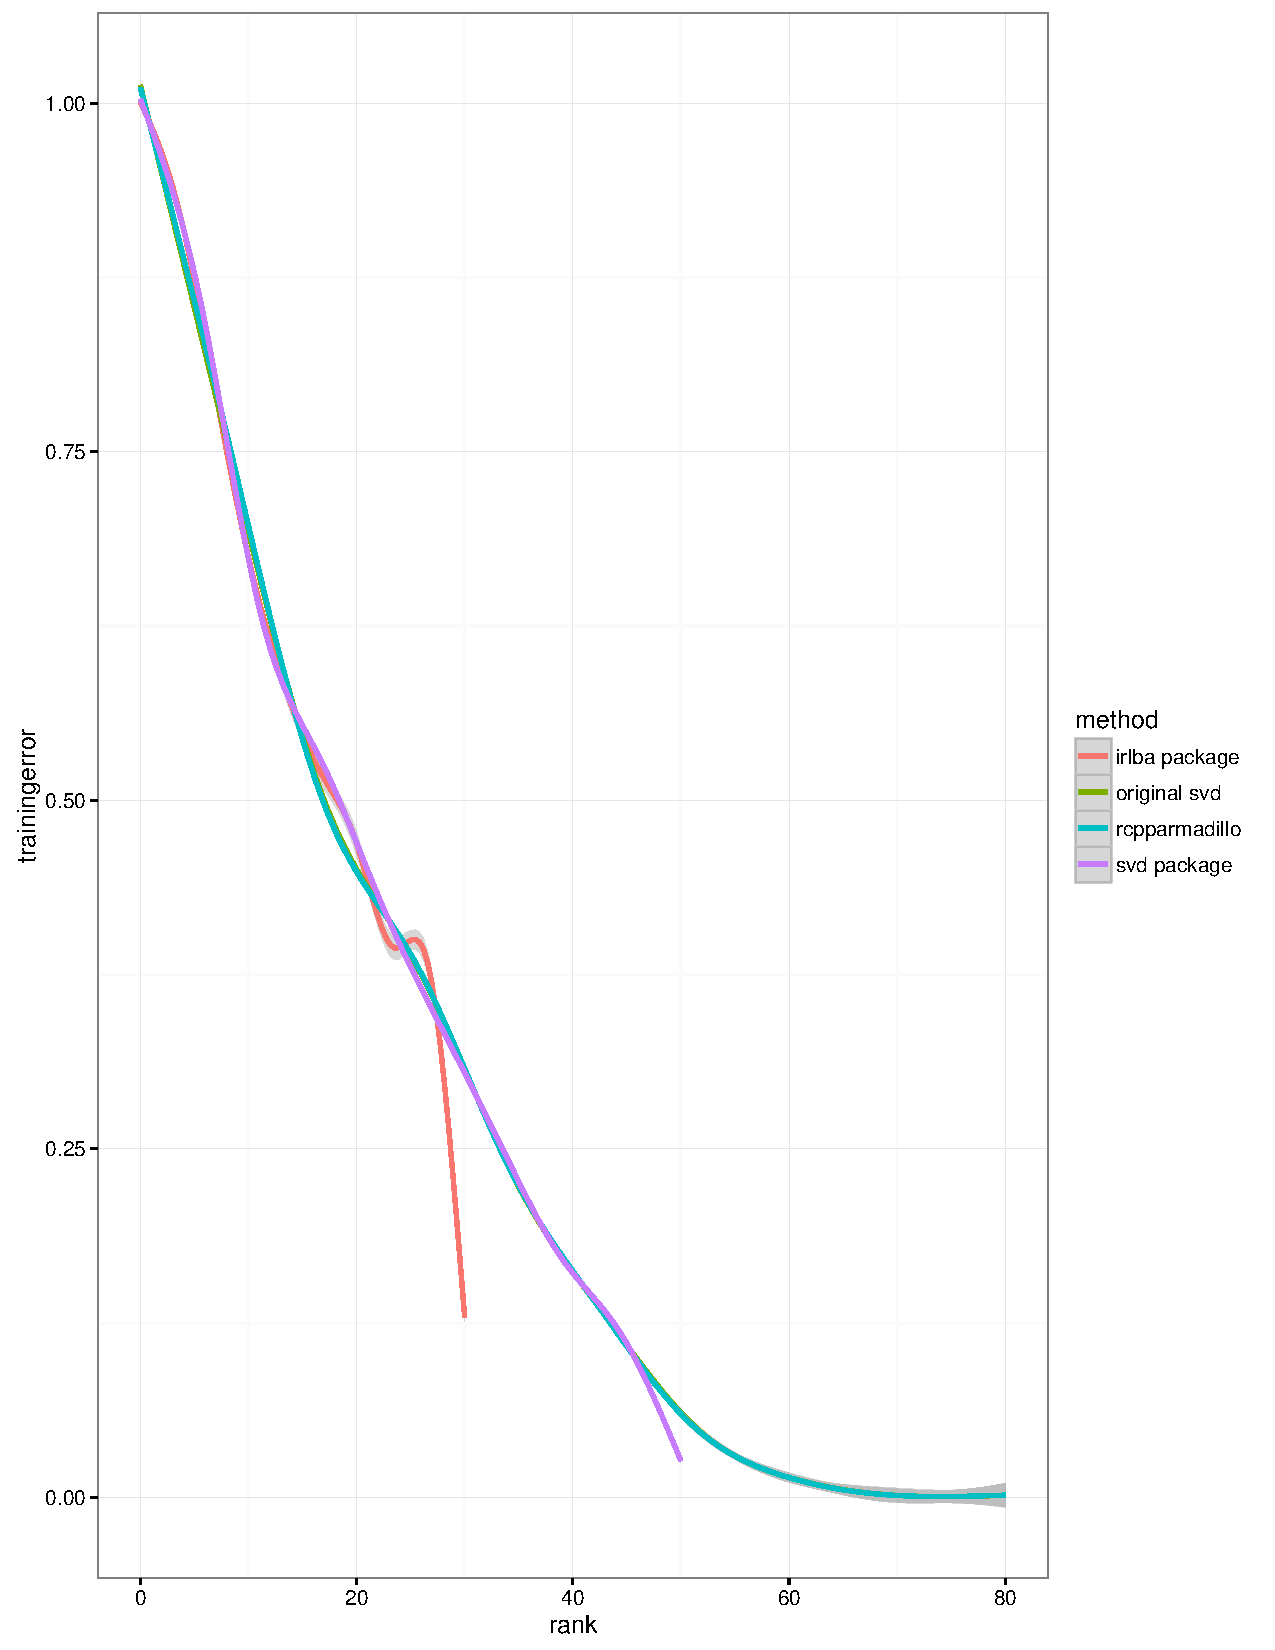
\includegraphics[width=0.45\textwidth]{trainingerror.pdf}}
  \caption{Compare the test error against the rank among the 4 methods with $p = 50\%, \mathrm{SNR} = 1, \textrm{true rank} = 10, m = n =100.$}\label{comparison_testerror}
\end{figure}

As we can see in the figures, the soft-impute using svd methods \verb|original svd| and \verb|rcpparmadillo| perform very similarly. While the method of \verb|irlba package| seems to have lowest Test error at some rank, but it seems fluctuate a lot. the methods \verb|original svd| and \verb|rcpparmadillo|. According to the training error, the method of \verb|irlba package| recovers a matrix with a relatively low rank which is closer to our true rank. So it has less evidence of overfitting.

Then we tried different properties of the generated matrix. Let $p = 0.3,0.5,0.8 ;\textrm{SNR} = 1,10; \textrm{true rank} = 5,10,20.$,then we get the table that compares the running time and test error among the 4 methods.

\begin{table}[!htp]
\centering
\caption{Performance of different methods for different problem instances in terms of test error and running time}
\vspace{0.5em}
\begin{tabular}{|c|c|c|c|c|c|c|c|c|c|c|}
\hline
time1&time2&time3&time4&error1&error2&error3&error4&true rank&SNR&$p$\\
\hline
2.1650&2.5915&1.3096&1.7030&0.2592&0.2592&0.2592&0.2592&5&1&0.3\\
\hline
2.0902&2.6631&1.4791&1.6333&0.4338&0.4338&0.4339&0.4338&10&1&0.3\\
\hline
2.0032&2.7237&1.6506&1.5678&0.6502&0.6502&0.6506&0.6502&20&1&0.3\\
\hline
1.9709&1.9810&0.6514&1.5437&0.0046&0.0046&0.0046&0.0046&5&10&0.3\\
\hline
1.9875&1.9486&0.6748&1.5096&0.0113&0.0113&0.0111&0.0113&10&10&0.3\\
\hline
2.0435&1.9584&0.6629&1.5443&0.0443&0.0432&0.0312&0.0443&20&10&0.3\\
\hline
2.8228&2.8239&1.3798&2.2199&0.3492&0.3492&0.3492&0.3492&5&1&0.5\\
\hline
2.6000&2.8008&1.6049&2.0534&0.5798&0.5798&0.5798&0.5798&10&1&0.5\\
\hline
2.4068&2.5195&1.7681&1.8531&0.7970&0.7970&0.7970&0.7970&20&1&0.5\\
\hline
2.8192&2.8098&0.9243&2.2188&0.0097&0.0097&0.0097&0.0097&5&10&0.5\\
\hline
2.7298&2.7674&0.9625&2.1510&0.0319&0.0319&0.0306&0.0319&10&10&0.5\\
\hline
2.6173&2.6013&0.9362&2.0141&0.1913&0.1896&0.1488&0.1913&20&10&0.5\\
\hline
4.1483&4.1360&2.3177&3.2476&0.7382&0.7382&0.7382&0.7382&5&1&0.8\\
\hline
4.4981&4.4856&2.5795&3.5294&0.9040&0.9040&0.9040&0.9040&10&1&0.8\\
\hline
3.8848&3.8947&2.4525&3.0592&0.9829&0.9829&0.9829&0.9829&20&1&0.8\\
\hline
3.9987&3.9948&1.5107&3.1125&0.1739&0.1739&0.1746&0.1739&5&10&0.8\\
\hline
4.1852&4.1783&1.9447&3.2685&0.5261&0.5261&0.5259&0.5261&10&10&0.8\\
\hline
4.6070&4.5803&2.4109&3.6193&0.8458&0.8458&0.8458&0.8458&20&10&0.8\\
\hline
\end{tabular}
\end{table}

This table shows that the minimum test errors among the 4 methods are quite similar, but the running time of method \verb|irlba package| is the shortest followed by \verb|rcpparmadillo|.

According to the comparison above, we'll use the method \verb|irlba package| in our application part, because it's the fastest one and in the figure it turns out to have minimum test error. We'll also use \verb|rcpparmadillo|, because it's also very fast and is more stable in the figure.

	\section{Application}
	\subsection{Lena}
	Based the comparison between these 4 implementations, we choose the \verb|original svd| in R to do the image imputing. The reason is that from {Figure} \ref{comparison_testerror} we can see the \verb|original svd| and \verb|rcpparmadillo| seems to be more steady than \verb|irlba package| (the gray region that represents confidence interval is smaller). Also these two methods seems to have smaller test error around the true matrix rank. Because the data for lena is not large, thus we do not care about the speed of implementations. And we can expect \verb|original svd| and \verb|rcpparmadillo| would give almost the same results from the comparison part, hence we choose to use \verb|orginal svd|. 

	First we randomly removed the 40\% of the lena and got an image with only 60\% being observed. Now we use the 60\% as our data to restore the image with soft-impute. In order to obtain an optimal restoration, we need to tune the parameter $\lambda$ in the soft-impute algorithm. The strategy we took is to further divide the data into two parts: 70\% as training data and 30\% as validation data. We did the imputation with a series of $\lambda$'s (we used $\lambda = 500, 490, \ldots, 10$). Then we compared the corresponding validation part of these imputed matrix with the true validation set. The error term we used is
	\begin{equation}\label{valid_error}
	\frac{\|P_{\Omega_{\rm validation}}(Z_{\rm true} - \hat{Z}_{\lambda})\|^2_{F}}{\|P_{\Omega_{\rm validation}} Z_{\rm true}\|_{F}^2}
	\end{equation}
	where $\Omega_{\rm validation}$ is the set of matrix entries that validation set has.

	We chose the $\lambda$ that gave us the smallest test error and applied soft-impute again on the whole data set with the optimal $\lambda$ we got. In this case, with the test error we defined, the optimal $\lambda$ we chose is $\lambda = 190$. 

	After we imputed the matrix, we wanted to see how close it is to the true one. We looked at the rank of recovered matrix and the true matrix, and also the error of the imputed one compared with the true one. The error we used is 
	\begin{equation} \label{test_error}
	\frac{\|P_{\Omega_{\rm test}}(Z_{\rm true} - \hat{Z}_{\lambda})\|_{F}^2}{\|P_{\Omega_{\rm test}}(Z_{\rm true})\|_F^2} 
	\end{equation}
	where $\Omega_{\rm test}$ is the set of matrix entries that test set has, which is the rest 40\% of the true lena image that is not taken as data.

	With the optimal $\lambda$, the rank of recovered matrix is
	\[\textrm{rank} (\hat{Z}_{\lambda_{\rm opt}}) = 77\]
	While the true rank is
	\[\textrm{rank}(Z_{\rm true}) = 254\]

	The test error of the imputed matrix when compared with the true matrix in the rest 40\% of the image is  
	\[\textrm{test error} = 0.031\]

	Finally, we compare the true image, incomplete image and the restored image visually, which is shown in Figure \ref{lena}.
	\begin{figure}[!htb]
    \centering
    \subfigure[true image]{
            
\includegraphics[width=1.8in]{lena_true.jpg}

    }
    ~ 
    \subfigure[incomplete image]{
        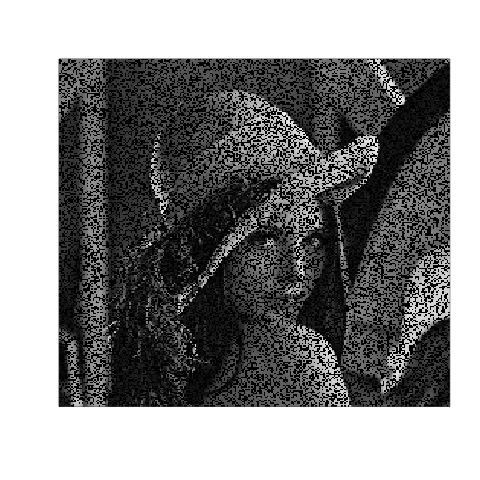
\includegraphics[width=1.8in]{lena_data.jpg}
}
     ~ 
    \subfigure[restored image]{
        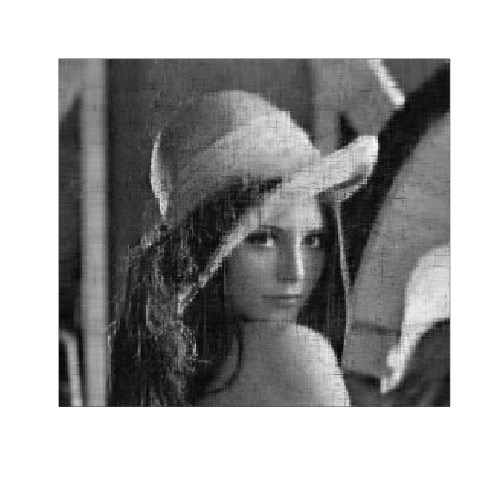
\includegraphics[width=1.8in]{lena_restored}
    }
    \caption{Visually comparing the imputed image with the true one}
    \label{lena}
\end{figure}
	
	We can see that the restored image is not so good. It is not like a natural image with good smoothness. Also the restored image has a much smaller rank than the true one. However, soft-impute is intended to impute low-rank matrix, and true image actually has a quite big rank. That might also be a reason why the final result is not good.

	\subsection{MovieLens}

	In this section, we use MovieLen 100K Dataset to apply our soft-impute algorithm. As the data set is not complete when we convert the original data into a matrix form, we need to divide it into three parts: 70\% as training set, 15\% as validation set and 15\% as test set. What we did is similar as we did in lena part. We first use the training set as observed entries to impute the matrix, then we compare the validation set with the corresponding entries of the imputed matrix. Again we use (\ref{valid_error}) as the error term and we pick the $\lambda$ with the smallest validation error. After we obtained the optimal $\lambda$, we use the 70\% training set and 15\% validation set combined as our data, or observed entries to impute the matrix. Then we compare the test set with the corresponding entries of the imputed matrix and calculate the test error using (\ref{test_error}). Besides, we calculated the RMSE of the imputed matrix with respect to the test set in corresponding parts. The RMSE formula is
	\begin{equation}
	\textrm{RMSE} = \sqrt{\frac{\|P_{\Omega_{\rm test}}(Z_{\rm true} - \hat{Z}_{\lambda_{\rm opt}})\|_{F}^2}{|\Omega_{\rm test}|}}
	\end{equation}

	As the dataset is pretty big, we chose \verb|irlba package| and \verb|rcpparmadillo| as two implementations to be applied to this dataset. There two implementations are relatively faster than others ,thus with the big dataset we could save a lot of time. 

	In choosing the optimal $\lambda$, as the big matrix takes time to impute, we used a strategy to find the optimal one using 3 grids of $\lambda$'s by assuming the test error as a function of $\lambda$ is unimodal. The first grid is $\lambda = 100, 90, \ldots, 10$ with step size 10. From this grid we can find the interval where the optimal $\lambda$ located. We found $\lambda  = 10$ was the smallest in this grid. Then we knew the optimal $\lambda$ is between $20$ and $0$. Then we used the second grid $\lambda = 19, 16, \ldots, 4, 1$ with step size 3. We found $\lambda = 13$ is the smallest in this grid. Then we tried the third grid $\lambda = 15, 14, 12, 11$. In this grid, $\lambda = 12$ gave us the smallest test error. But comparing it with the test error when $\lambda = 13$, we found the test error for $\lambda =13$ was smaller. Hence, the optimal $\lambda$ we chose is $\lambda = 13$. 

	The time it took in each $\lambda$ grid, the best $\lambda$ for that grid and the corresponding validation error for that best $\lambda$ for both methods are given below.

	\begin{table}[!htb]
	\centering
	\caption{Time, best $\lambda$, validation error for two methods in three grids}
	\vspace{0.5em}
	\label{3grids}
		\begin{tabular}{|l|l|l|l|l|}
\hline
                                   & method               & time      & best $\lambda$ & validation error \\ \hline
\multirow{2}{*}{$1_{\rm st}$ grid} & \verb|irlba package| & 6278.067  & 10             & 0.07842399       \\ \cline{2-5} 
                                   & \verb|rcpparmadillo| & 43121.128 & 10             & 0.07840086       \\ \hline
\multirow{2}{*}{$2_{\rm nd}$ grid} & \verb|irlba package| & 12487.161 & 13             & 0.07705321       \\ \cline{2-5} 
                                   & \verb|rcpparmadillo| & 35947.462 & 13             & 0.07707266       \\ \hline
\multirow{2}{*}{$3_{\rm rd}$ grid} & \verb|irlba package| & 3673.131  & 12             & 0.07710168       \\ \cline{2-5} 
                                   & \verb|rcpparmadillo| & 20142.322 & 12            & 0.07715054       \\ \hline
\end{tabular}
	\end{table}

	From Table \ref{3grids}, we can see the method \verb|irlba  package| is a lot faster. However the best $\lambda$ and validation error they got for each grid are almost the same.

	Using the optimal $\lambda = 13$, we obtained the imputed matrix and compare the corresponding test set entries in the matrix with test set. The test error and RMSE we got is shown below.
	\begin{table}[!htb]
	\centering
		\caption{Test error and RMSE with respect to two methods}
		\vspace{0.5em}
		\begin{tabular}{|l|l|l|l|l|}
		\hline
			& optimal $\lambda$ & test error & RMSE \\ \hline
		\verb|irlba package| & 13 & 0.07705321 & 1.0283 \\ \hline
		\verb|rcpparmadillo| & 13 & 0.07707266 & 1.0284 \\ \hline
		\end{tabular}
	\end{table}

	The two methods gave almost the same test error and RMSE, thus the major difference between is the speed. In the case of large dataset, \verb|irlba package| is much more efficient.

	\newpage

	\bibliographystyle{unsrt}
	\bibliography{reference}

	\newpage

	\begin{appendices}
	\section{Appendix: Codes for final project}

	C LAPACK soft-impute implementation:

	\lstinputlisting[language = C]{../soft_impute.c}
	\end{appendices}

	C part for RCpp Armadillo implementation:

	\lstinputlisting[language = C]{../armadillo_svd.cpp}

	All functions used in comparison and application part, includin four implementations of soft-impute:

	\lstinputlisting[language = R]{../fpfunctions2.R}

	Plot part of comparison:

	\lstinputlisting[language = R]{../comparison_graph.R}

	Table part of comparison:

	\lstinputlisting[language = R]{../comparison_test.R}

	Lena:

	\lstinputlisting[language = R]{../lena_comparison.R}

	The first grid part of $\lambda$ selection in MovieLens ($\lambda = 100, 90, \ldots, 10$):

	Using \verb|irlba package|

	\lstinputlisting[language = R]{../movie_comparison_irlba_server.R}

	Using \verb|rcpparmadillo|
	
	\lstinputlisting[language = R]{../movie_c_cpp_server.R}

	Imputing matrix using optimal $\lambda$ and getting test error and RMSE:

	\lstinputlisting[language = R]{../impute_using_optimal_lambda.R}

	\lstinputlisting[language = R]{../RMSE.R}





	
	\end{document}